\begin{exercises} 
\item Let $f$ and $g$ be differentiable functions for which the following information is known:  $f(2) = 5$, $g(2) = -3$, $f'(2) = -1/2$, $g'(2) = 2$.
\ba
	\item Let $h$ be the new function defined by the rule $h(x) = 3f(x) - 4g(x)$.  Determine $h(2)$ and $h'(2)$.
	\item Find an equation for the tangent line to $y = h(x)$ at the point $(2,h(2))$.
	\item Let $p$ be the function defined by the rule $p(x) = -2f(x) + \frac{1}{2}g(x)$.  Is $p$ increasing, decreasing, or neither at $a = 2$?  Why?
	\item Estimate the value of $p(2.03)$ by using the local linearization of $p$ at the point $(2,p(2))$.
\ea
\begin{exerciseSolution}
\end{exerciseSolution}
\item Consider the functions $r(t) = t^t$ and $s(t) = \arccos(t)$, for which you are given the facts that $r'(t) = t^t(\ln(t) + 1)$ and $s'(t) = -\frac{1}{\sqrt{1-t^2}}$.  Do not be concerned with where these derivative formulas come from.  We restrict our interest in both functions to the domain $0 < t < 1$.
\ba
	\item Let $w(t) = 3t^t - 2\arccos(t)$.  Determine $w'(t)$.
	\item Find an equation for the tangent line to $y = w(t)$ at the point $(\frac{1}{2}, w(\frac{1}{2}))$.
	\item Let $v(t) = t^t + \arccos(t)$.  Is $v$ increasing or decreasing at the instant $t = \frac{1}{2}$?  Why?
\ea
\item Let functions $p$ and $q$ be the piecewise linear functions given by their respective graphs in Figure~\ref{F:2.1.Ez3}.  Use the graphs to answer the following questions.
\begin{figure}[h]
\begin{center}
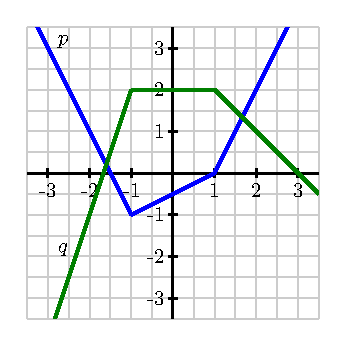
\includegraphics{figures/2_1_Ez3.eps}
\caption{The graphs of $p$ (in blue) and $q$ (in green).} \label{F:2.1.Ez3}
\end{center}
\end{figure}
\ba
	\item At what values of $x$ is $p$ not differentiable?  At what values of $x$ is $q$ not differentiable? Why?
	\item Let $r(x) = p(x) + 2q(x)$.  At what values of $x$ is $r$ not differentiable? Why?
	\item Determine $r'(-2)$ and $r'(0)$.
	\item Find an equation for the tangent line to $y = r(x)$ at the point $(2,r(2))$.
\ea

\item Let $f(x) = a^x$.  The goal of this problem is to explore how the value of $a$ affects the derivative of $f(x)$, without assuming we know the rule for $\frac{d}{dx}[a^x]$ that we have stated and used in earlier work in this section.
\ba
	\item Use the limit definition of the derivative to show that
	$$f'(x) = \lim_{h \to 0} \frac{a^x \cdot a^h - a^x}{h}.$$
	\item Explain why it is also true that
	$$f'(x) = a^x \cdot \lim_{h \to 0} \frac{a^h - 1}{h}.$$
	\item Use computing technology and small values of $h$ to estimate the value of 
	$$L = \lim_{h \to 0} \frac{a^h - 1}{h}$$
	when $a = 2$.  Do likewise when $a = 3$.
	\item Note that it would be ideal if the value of the limit $L$ was $1$, for then $f$ would be a particularly special function:  its derivative would be simply $a^x$, which would mean that its derivative is itself.  By experimenting with different values of $a$ between $2$ and $3$, try to find a value for $a$ for which 
	$$L = \lim_{h \to 0} \frac{a^h - 1}{h} = 1.$$
	\item Compute $\ln(2)$ and $\ln(3)$.  What does your work in (b) and (c) suggest is true about $\frac{d}{dx}[2^x]$ and $\frac{d}{dx}[2^x]$.
	\item How do your investigations in (d) lead to a particularly important fact about the number $e$?
\ea

\end{exercises}
\afterexercises